\documentclass[a4paper, 12pt]{article}
\usepackage{graphicx}
\usepackage{amsmath, amssymb}
\usepackage{hyperref}
\usepackage{enumitem}
\usepackage[ngerman]{babel}
\usepackage[utf8]{inputenc}

\setlength{\parindent}{0pt}

\title{Abgabe 1 für Computergestützte Methoden}
\author{Gruppe 40, Elias Penner 4362765, Julian Kulke 4346397 }
\date{November 2024}

\begin{document}

\maketitle

\tableofcontents
\newpage

\section{Der Zentrale Grenzwertsatz}
Der zentrale Grenzwertsatz (ZGS) ist ein fundamentales Resultat der Wahrscheinlichkeitstheorie, das die Verteilung von Summen unabhängiger, identisch
verteilter \textit{(i.i.d.)} Zufallsvariablen (ZV) beschreibt. Er besagt, dass unter bestimmten Voraussetzungen die Summe einer großen Anzahl solcher ZV annähernd
normalverteilt ist, unabhängig von der Verteilung der einzelnen ZV. Dies ist besonders nützlich, da die Normalverteilung gut untersucht und mathematisch handhabbar ist.

\subsection{Aussage}
Sei \(X_1, X_2,\ldots, X_n\) eine Folge von \textit{i.i.d.} ZV mit dem Erwartungswert $\mu = \mathbb{E}(X_i)$ und der Varianz \(\sigma^2 =Var(X_i) \), wobei \(0< \sigma^2 < \infty\) gelte. Dann konvergiert die standardisierte Summe \(Z_n\) dieser ZV für \(n \rightarrow \infty\) in Verteilung gegen eine
Standardnormalverteilung:
\footnote{Der zentrale Grenzwertsatz hat verschiedene Verallgemeinerungen. Eine davon ist der \textbf{Lindeberg-Feller-Zentrale-Grenzwertsatz} \cite[Seite 328]{Wahrscheinlichkeitstheorie_Achim_Klenke}, der schwächere Bedingungen an
die Unabhängigkeit und die identische Verteilung der ZV stellt.}


\[Z_n = \frac{\sum_{i=1}^n X_i-n\mu}{\sigma \sqrt{n}} \xrightarrow{d} \mathcal{N}(0, 1). \tag{1} \label{Formel 1}\]


Das bedeutet, dass für große \(\ n\) die Summe der ZV näherungsweise normalverteilt
ist mit Erwartungswert \(n\mu\) und Varianz \(n\sigma^2\):

\[\sum_{i=1}^n X_i \sim \mathcal{N}(n\mu, n\sigma^2). \tag{2} \label{Formel 2}\]

\subsection{Erklärung der Standardisierung}
Um die Summe der ZV in eine Standardnormalverteilung zu transformieren, subtrahiert man den Erwartungswert \(n\mu\) und teilt durch die Standardabweichung \(\sigma \sqrt{n}\). Dies führt zu der obigen Formel (\ref{Formel 1}). Die Darstellung (\ref{Formel 2}) ist für \(n \rightarrow \infty\) nicht wohldefiniert.

\subsection{Anwendung}Der ZGS wird in vielen Bereichen der Statistik und der Wahrscheinlichkeitstheorie angewendet. Typische Beispiele sind:

\newpage
\textbf{Simulationen in der Finanzmathematik}
\begin{itemize}
    \item
    \textbf{Anwendung:} Finanzmodelle zur Risikobewertung setzen oft voraus, dass die Summe kleiner täglicher Preisänderungen eines Aktienportfolios einer Normalverteilung folgt.

    \item 
    \textbf{Beispiel:} In der Optionsbewertung wird angenommen, dass die Renditen eines Wertpapiers über einen bestimmten Zeitraum normalverteilt sind, obwohl die täglichen Preisänderungen nicht direkt dieser Verteilung folgen.
\end{itemize}

\textbf{Hypothesentests und Konfidenzintervalle}
\begin{itemize}
    \item
    \textbf{Anwendung:} Viele statistische Tests (z.B. t -Tests,  z -Tests) basieren auf der Annahme, dass die Stichprobenmittelwerte normalverteilt sind, was durch den ZGS gerechtfertigt ist.

    \item
    \textbf{Beispiel:} Beim Testen, ob ein neues Medikament die durchschnittliche Genesungszeit verkürzt, wird der Mittelwert der Genesungszeiten aus Stichproben analysiert. Der ZGS erlaubt die Verwendung von Normalverteilungsannahmen.
\end{itemize}

\newpage

\section{Bearbeitung zur Aufgabe 1}
\section*{Thema: Datenverabeitung}
\subsection{Aufgabe 1.1}
Nach dem Importieren des Datensatzes in Excel wurde ersichtlich, dass die gegebene Tabelle unsortiert vorliegt, d.h. alle gegebenen Daten in einer Tabellen-Spalte aufgeführt sind. Daher ist die Tabelle in ihrer aktuellen Form ungeeignet, um mittels der Sortierfunktion konkrete Daten zu ermitteln und mit ihr zu arbeiten.
\newline
Um mit der gegebenen Tabelle weiterarbeiten zu können, muss diese erst sortiert werden. Dabei müssen allen Überkategorien samt ihrer Werte, wie „station“, „date“, etc., eigene Spalten zugewiesen werden. Des Weiteren sind in der Ausgangstabelle die Datensätze für alle Gruppen hinterlegt. Für uns sind jedoch nur die Datensätze für Gruppe 40 relevant, weshalb wir die Tabelle zusätzlich nach der Gruppe filtern müssen.

\subsection{Aufgabe 1.3}
Die gegebenen Werte der Tabelle müssen vorerst auf einzelne Spalten aufgeteilt werden. Da die einzelnen Datenkategorien durch Kommas getrennt sind, kann die Funktion \textit{Text in Spalten} in Excel verwendet werden, um die einzelnen Überkategorien der Tabelle zu sortieren.

\begin{enumerate}
    \item \textit{Text in Spalten Funktion} auswählen.
    \item Dateitypeinstellung auf \textit{Getrennt} lassen, da unser Datensatz durch Kommas getrennt ist.
    \item \textit{Komma} als Trennzeichen auswählen.
    \item Datenformat der Spalten im letzten Schritt auf \textit{Standard} belassen und auf \textit{Fertig stellen} klicken.
\end{enumerate}

Die Tabelle ist nun so sortiert, sodass alle Überkategorien in eigenen Spalten aufgeführt werden.\newline Danach sortieren wir die Spalte J mit der Filterfunktion von Excel nach Größe (absteigend): \texttt{Filter > Pfeil an Spalte auswählen > Nach Größe sortieren (absteigend) > Markierung erweitern > Sortieren}
\\
\newline
Nach dem Sortieren ist der höchste Wert mit 83 Grad Fahrenheit ersichtlich.

\newpage

\begin{figure}[!htb]
\centering
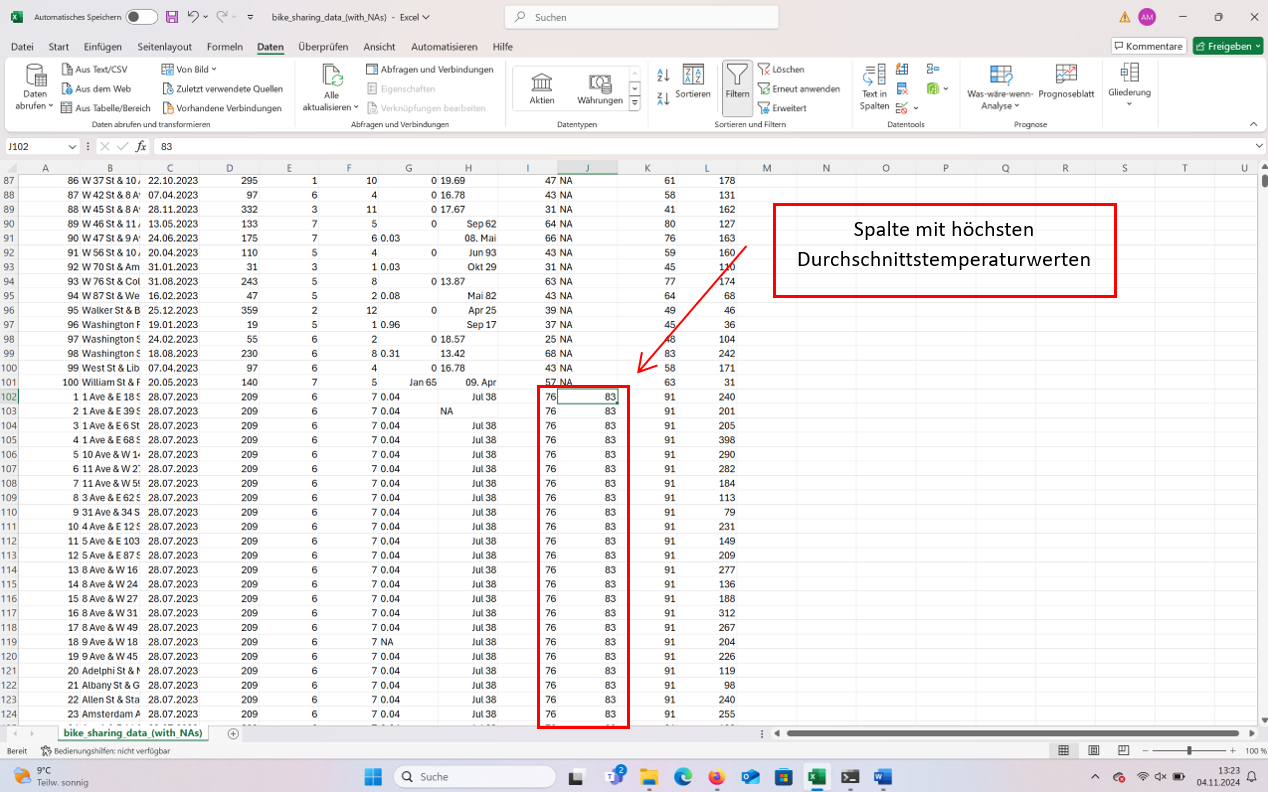
\includegraphics[scale=.4]{Screenshot 2024-11-26 201311}
\caption{Screenshot Excel-Tabelle}
\label{fig:Screenshot Excel-Tabelle}
\end{figure}

Die sortierten Fahrenheit-Werte müssen in Excel in Grad Celsius umgerechnet werden. Dafür erstellen wir eine neue Spalte M: \[\texttt{M: average\_temperature\_Grad\_Celsius}\] In diese Spalte schreiben wir den Befehl: \[\texttt{=(J2-32)*5/9}\] \newline \texttt{J2} ist hierbei der Spalten- und Zeilenverweis, den Excel nutzt, um die Fahrenheit Werte aus Spalte J in Spalte M zu übernehmen. \newline \texttt{(x-32)*5/9} ist der Umrechnungsfaktor von Fahrenheit in Grad Celsius. Diese Formel wird nun durch einen Doppelklick auf das Ausfüllkästchen in alle darunter liegenden Zeilen kopiert. Auch wenn die restlichen Tabellenwerte umsortiert werden, würde die Umrechnung in Spalte M weiterhin funktionieren.

\newpage
\begin{figure}[!htb]
\centering
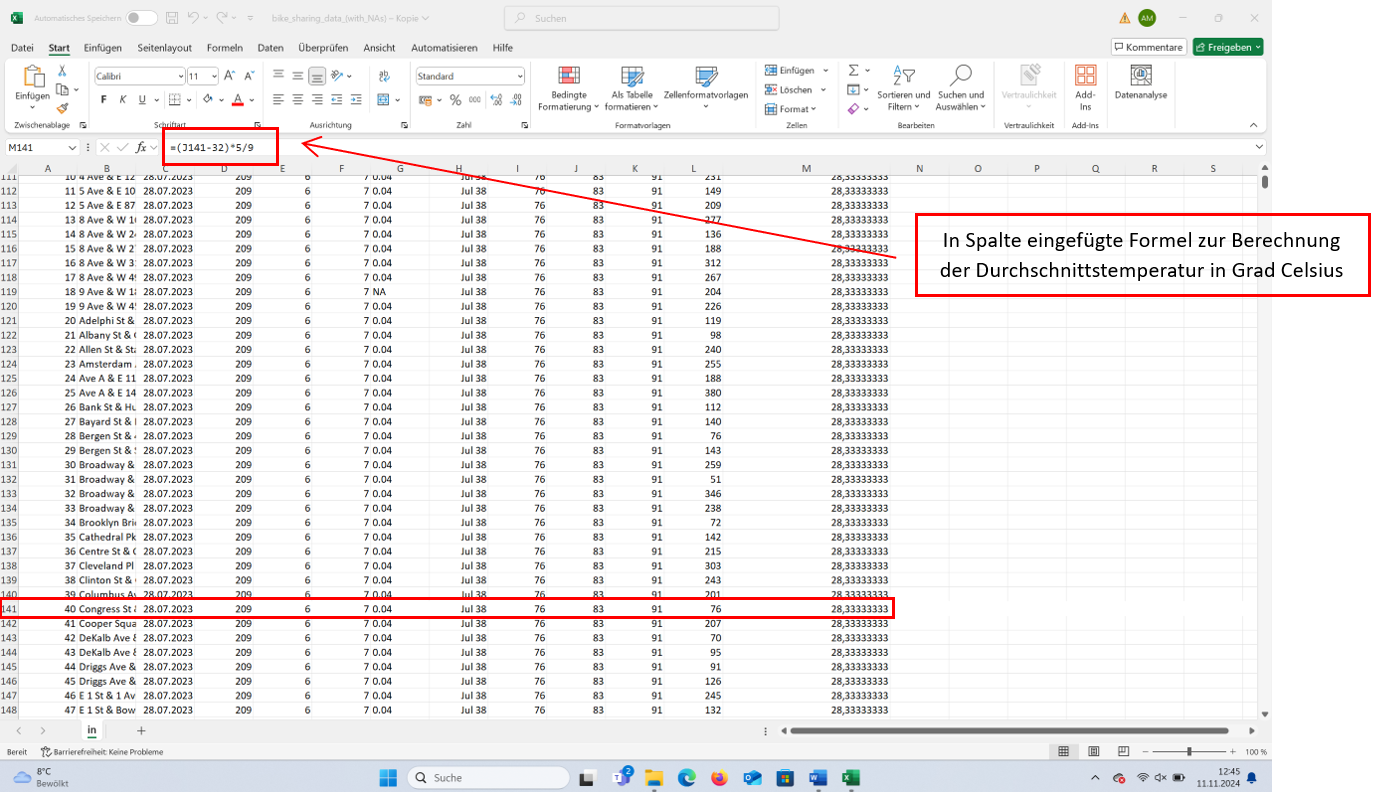
\includegraphics[scale=.4]{Screenshot 2024-11-26 201341}
\caption{Screenshot Excel-Tabelle}
\label{fig:Screenshot Excel-Tabelle}
\end{figure}

Zuletzt filtern wir die Daten so, dass nur noch die Daten für Gruppe 40 vorliegen. Dies machen wir ebenfalls mit der Filterfunktion. Dafür markieren wir alle Daten mittels \texttt{Strg A} und wählen unter dem \texttt{Daten-Reiter} die Filter Funktion aus. Danach wählen wir in der Spalte „Group“ den kleinen Pfeil auf der rechten Seite aus und selektiere im Auswahlmenü ausschließlich die Zahl 40. Nun stehen nur noch alle sortierten Werte von Gruppe 40 in der Tabelle.

\newpage
\begin{figure}[!htb]
\centering
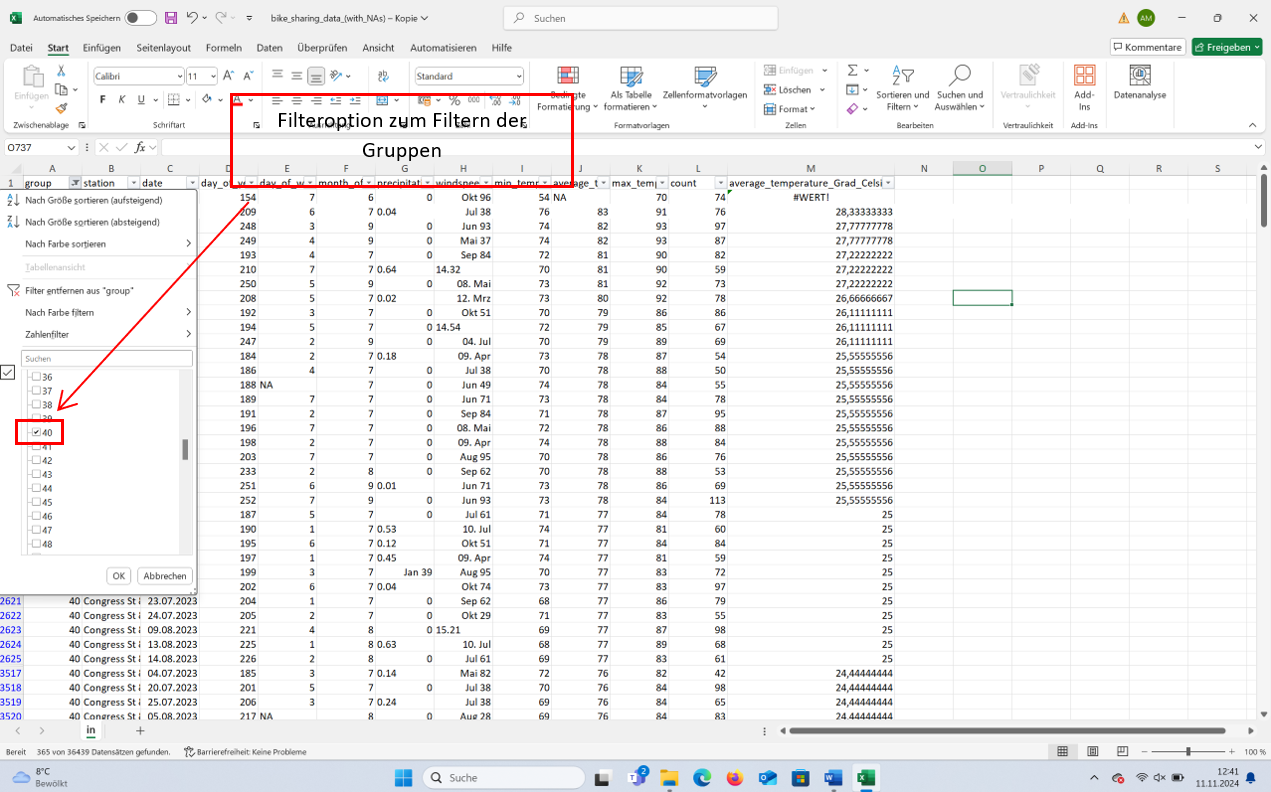
\includegraphics[scale=.4]{Screenshot 2024-11-26 201403}
\caption{Screenshot Excel-Tabelle}
\label{fig:Screenshot Excel-Tabelle}
\end{figure}

\begin{figure}[!htb]
\centering
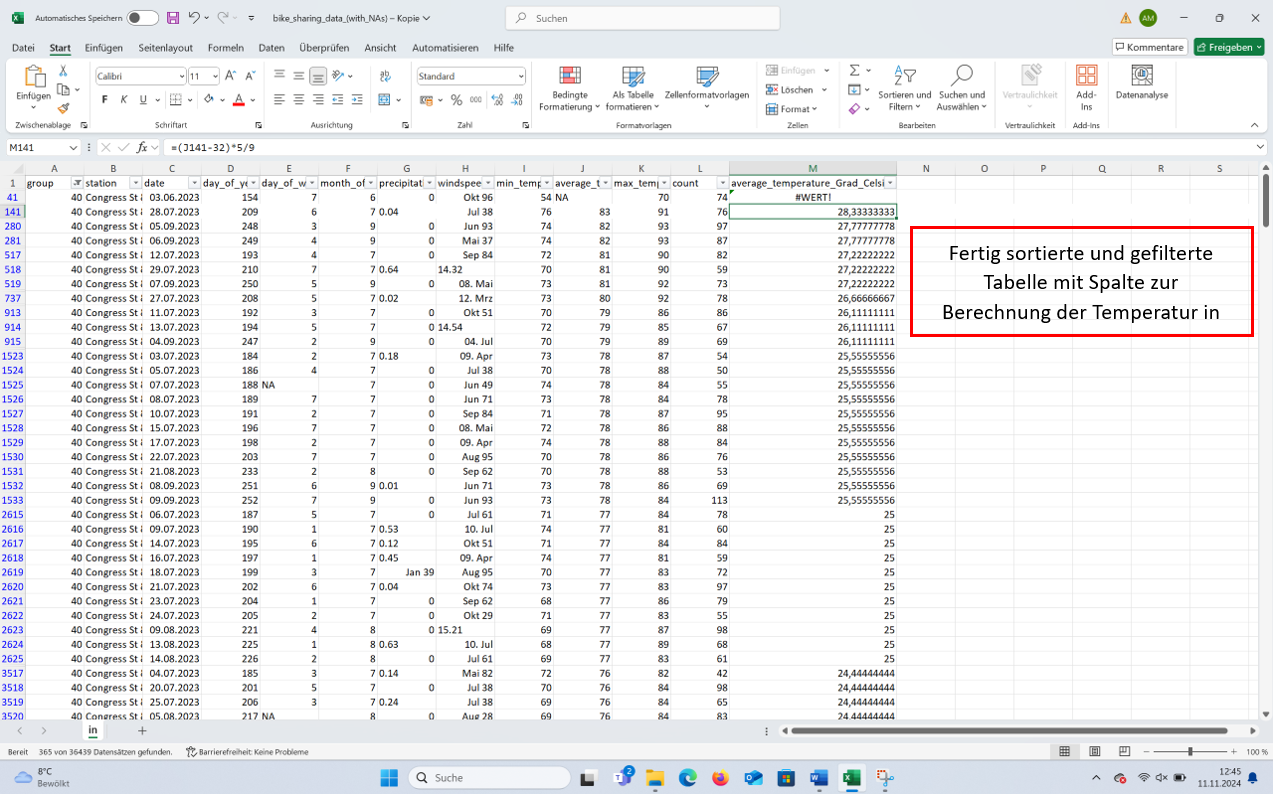
\includegraphics[scale=.4]{Screenshot 2024-11-26 201421}
\caption{Screenshot Excel-Tabelle}
\label{fig:Screenshot Excel-Tabelle}
\end{figure}

\newpage
\subsection*{Thema: Datenhaltung}
\subsection{Aufgabe 1.2}
Stationen (\underline{StationID\#} , Name)
\\

Wetter Daten (\underline{GroupID\#}, StationID\# , Datum, count, precepitation, windspeed, min temp, avg temp, max temp, day of year, day of week, month of year)

\subsection{Aufgabe 1.3}
Zum Ausführen des SQL-Codes nutzen wir die Kommandozeile mit der SQLite Erweiterung.
\\

\textbf{Code:} \newline
\textbf{Tabelle Station:}
\begin{verbatim}
CREATE TABLE Stationen ( 
    station_id INTEGER PRIMARY KEY AUTOINCREMENT,
    station_name TEXT UNIQUE 
);
\end{verbatim}

\textbf{Tabelle Wetterdaten:}
\begin{verbatim}
CREATE TABLE Wetter_Daten (
    id INTEGER PRIMARY KEY AUTOINCREMENT,
    group_id INTEGER,
    station_id INTEGER,
    date DATE,
    day_of_year INTEGER,
    day_of_week INTEGER,
    month_of_year INTEGER,
    precipitation FLOAT,
    windspeed FLOAT,
    min_temperature INTEGER,
    average_temperature INTEGER,
    max_temperature INTEGER,
    count INTEGER,
    FOREIGN KEY (station_id) REFERENCES station(station_id)
);    
\end{verbatim}



\newpage
\subsection{Aufgabe 1.4}
Um die Daten aus unserem CSV-Datensatz in SQL zu laden, erstellen wir zunächst mit dem Befehl CREATE TABLE Datenimport eine Temporäre Tabelle, in die der Gesamte CSV-Datensatz, in seiner Ursprünglichen Form, geladen wird. Im nächsten Schritt werden die Spalten aus der Temporären Tabelle in  die voher von uns erstellten Tabellen, Tabelle Station und Tabelle Wetterdaten aufgeteilt. Dafür werden als erstes die zugehörigen Daten mit dem Befehl INSERT OR IGNORE INTO Stationen in die Stationen Tabelle eingefügt. Zu dem INSERT-Befehl wird zusätzlich der IGNORE-Befehl verwendet, damit es keine doppleten Einträge in der Stationen Tabelle gibt. Mit dem SELECT-Befehl geben wir an, welche Daten in die Tabelle eingefügt werden sollen. Das gleiche machen wir auch für unsere zweite Tabelle Wetter Daten. Zum Schluss wird mit dem Befehl DROP TABLE Import die von uns zu Beginn erstellte Temporäre Tabelle gelöscht. Diese wird jetzt nicht mehr benötigt und würde nur zusätzlich Speicher verbrauchen, da unsere Daten nun Zugeorndet in den Beiden Tabellen Stationen und Wetterdaten vorliegen. Im Anschluss können nun, in Aufgabe 5, beliebige Daten mit einem SELECT-Befehl aus der Tabelle abgefragt werden.

\newpage
\begin{verbatim}
CREATE TABLE Datenimport (
    group_id INTEGER,
    station_name TEXT,
    date DATE,
    day_of_year INTEGER,
    day_of_week INTEGER,
    month_of_year INTEGER,
    precipitation FLOAT,
    windspeed FLOAT,
    min_temperature INTEGER,
    average_temperature INTEGER,
    max_temperature INTEGER,
    count INTEGER
);

.mode csv
.headers on
.import "bike_sharing_data_(with_NAs).csv" Datenimport

INSERT OR IGNORE INTO Stationen (station_name)
SELECT DISTINCT station_name
FROM Datenimport;

INSERT INTO Wetter_Daten (
    group_id, station_id, date, day_of_year, day_of_week, month_of_year,
    precipitation, windspeed, min_temperature, average_temperature,
    max_temperature, count
)
SELECT 
    t.group_id,
    s.station_id,
    t.date,
    t.day_of_year,
    t.day_of_week,
    CASE WHEN t.month_of_year = 'NA' THEN NULL ELSE t.month_of_year END,
    t.precipitation,
    t.windspeed,
    t.min_temperature,
    t.average_temperature,
    t.max_temperature,
    t.count
FROM Datenimport t
JOIN Stationen s ON t.station_name = s.station_name;

DROP TABLE Datenimport;
\end{verbatim}

\subsection{Aufgabe 1.5}
\begin{verbatim}
SELECT
    ROUND((MAX(CAST(average_temperature AS 
    FLOAT)) - 32) * 5/9, 2) AS
    highest_average_temperature_celsius 
FROM
    Wetter_Daten
WHERE
    group_id = 40;
\end{verbatim}

\begin{figure}[!htb]
\centering
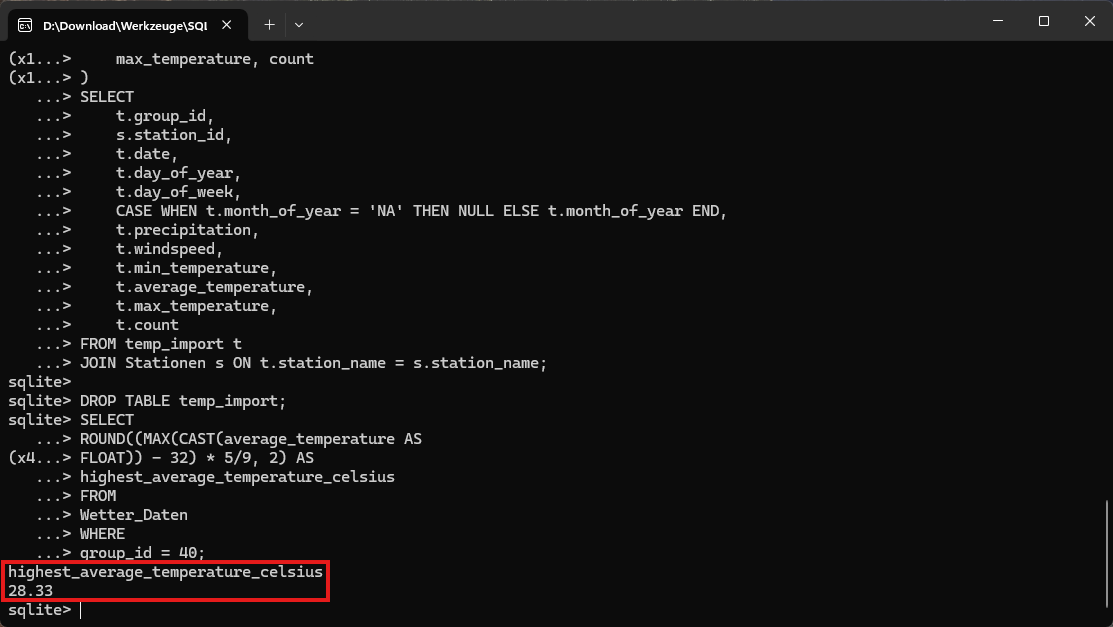
\includegraphics[scale=.4]{Screenshot 2024-12-01 185857}
\caption{Screenshot Kommandozeile Ergebnis}
\label{fig:Screenshot Kommandozeile}
\end{figure}

Als Ergebnis für die höchste Durchschnittstemperatur ehrhalten wir, identisch zu unserem Excel-Ergbnis, einen Wert von 28,33 Grad Celsius.

\newpage
\section{GitHub Abgabe}
\textbf{Dauerlink zum GitHub repositorie:} \newline
\url{https://github.com/JulianKlk/Abgabe_Computer_Gestuetzte_Methoden}

\newpage
\begin{thebibliography}{9}
\bibitem{Wahrscheinlichkeitstheorie_Achim_Klenke}
Achim Klenke. \textit{Wahrscheinlichkeitstheorie}. Springer, 3. Auflage, 2013.
\end{thebibliography}

\end{document}
